\chapter{Análise do Software} 
\label{sec:tp1}

\section{Teste de Software}
Não se pode garantir que todo software funcione corretamente, sem a presença de erros, visto que os mesmos muitas vezes possuem um grande número de estados com fórmulas, atividades e algoritmos complexos. Falhas podem ser originadas por diversos motivos. Por exemplo, a especificação pode estar errada ou incompleta, ou pode conter requisitos impossíveis de serem implementados, devido a limitações de hardware ou software. A implementação também pode estar errada ou incompleta, como um erro de um algoritmo. Portanto, uma falha é o resultado de um ou mais defeitos em algum aspeto do sistema.
O teste de software pode ser visto como uma parcela do processo de qualidade de software e quando falamos em testes de software devemos sempre lembrar que estes são divididos em diversos tipos, de acordo com seu objetivo particular, de seguida apresentamos os testes desenvolvidos de acordo com o seu tipo para a aplicação em estudo. 

\subsection{Testes Unitários}
O teste unitário ou de unidade é uma modalidade de testes que se concentra na verificação da menor unidade do projeto de software. É realizado o teste de uma unidade lógica, com uso de dados suficientes para se testar apenas a lógica da unidade em questão. Em sistemas construídos com uso de linguagens orientadas a objetos, como Java, essa unidade pode ser identificada como um método, uma classe ou mesmo um objeto.

Assim, o teste unitário  testa o menor dos componentes de um sistema de maneira isolada. Cada uma dessas unidades define um conjunto de estímulos (chamada de métodos), e de dados de entrada e saída associados a cada estímulo. As entradas são parâmetros e as saídas são o valor de retorno, exceções ou o estado do objeto.

Esse tipo de teste é de responsabilidade do próprio desenvolvedor durante a implementação do sistema, isto é, após codificar uma classe, por exemplo, ele planeja, codifica e executa o teste de unidade.

Os testes de unidade são considerados o estagio inicial da cadeia de testes a qual um software pode ser submetido. Essa categoria de testes não atende a testar toda a funcionalidade de uma aplicação, que fica a cargo de outros testes, como de integração ou de performance.

\subsubsection*{JUnit} 
O JUnit possibilita a criação das classes de testes. Estas classes contêm um ou mais métodos para que sejam realizados os testes, podendo ser organizados de forma hierárquica, de forma que o sistema seja testado em partes separadas, algumas integradas ou até mesmo todas de uma só vez. Além disso, esta framework tem como objetivo facilitar a criação de casos de teste, além de permitir escrever testes que retenham seu valor ao longo do tempo, ou seja, que possam ser reutilizáveis.

\subsubsection*{Testes realizados para a UMER} 
O primeiro passo foi testar se os métodos mais relevantes da classe \texttt{cliente} estavam corretamente implementadas de modo a verificar se a classe estava vulnerável a determinadas falhas. Assim, foi criada a classe \texttt{atorTeste} que realiza os seguintes testes:

\begin{itemize}
    \item \texttt{testarRegistaViagem()} - verifica se quando uma viagem é registada ela fica registada no histórico do ator
    
    \item \texttt{testarMaiorDesvio()} - verifica se quando se tenta invocar métodos sobre viagens e não existe nenhuma viagem registada se é lançada a excepção \texttt{NenhumaViagemException}
    
    \item \texttt{public void testarEquals()} - verifica se o método equals da classe \texttt{ator} está bem implementado
    
    \item \texttt{testarViagemEntreDatas()} - verifica se o método \texttt{viagemEntreDatas} se encontra corretamente implementado
\end{itemize}

De seguida fizeram-se alguns testes sobre a classe \texttt{Coordenada}, nomeadamente sobre os métodos mais relevantes a mesma:

\begin{itemize}
    \item \texttt{testarEquals()} - verifica através de vários testes se o método \texttt{equals} está bem implementado
    
    \item \texttt{testarDistancia()} - verifica se o método que calcula a distância entre duas coordenadas é corretmente calculada
\end{itemize}

Por último realizaram-se testes à classe \texttt{motorista}, nomeadamente aos métodos mais complexos, uma vez que os restantes métodos das outras classes correspondiam apenas a métodos \texttt{get} e \texttt{set} que por uma inspeção do código se verificou estarem bem implementados. 

\begin{itemize}
    \item \texttt{testarPrecoViagem()} - verifica se o preço de uma viagem é corretamente calculado. Ao executar este teste verificamos que esta classe está vulnerável a um erro pois aceita um número negativo para o preço e devolve um resultado errado

    \item \texttt{testarAtualizaDados()} - este teste verifica se os dados são atualizados quando o motorista faz uma viagem
    
    \item \texttt{testarTotalFaturado()} - verifica se o método \texttt{registaViagem} está a funcionar, nomeadamente se o total faturado pelo motorista após o registo da viagem é atualizado quando se regista uma nova viagem
\end{itemize}


\subsection{Cobertura}

O Cobertura é  uma ferramenta para calcular a percentagem de código coberta pelos códigos criados. Pode ser usado, por exemplo, para detetar partes do código que não estão a ser testadas.

\begin{figure}[H]
    \centering
    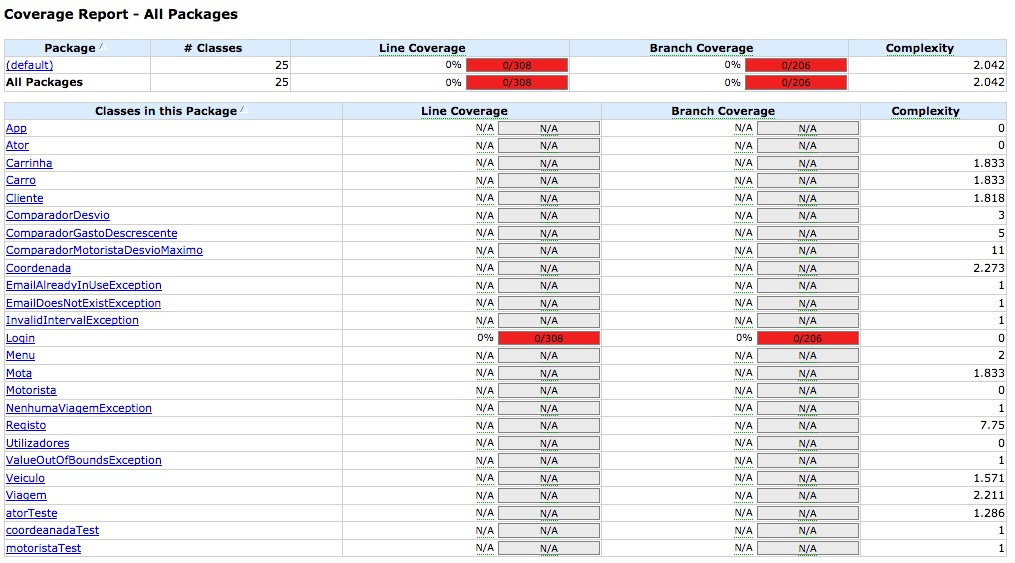
\includegraphics[scale=0.5]{tex/img/cobertura.jpg}
    \caption{Relatório do Cobertura}
    \label{fig:cobertura}
\end{figure}

Foi importante correr o Cobertura para ser possível o grupo ter uma melhor perceção da percentagem de código coberta pelos testes anteriormente explicitados.

\section{Análise do Código}

Foram usadas algumas técnicas exploradas durante as aulas para detetar e corrigir os bad smells, analisando assim a performance e correção do código.

\subsection{Bad Smells}

Em \emph{Software Engineering} , um bad smell é uma designação para um excerto de código que apesar de não estar errado tecnicamente nem impedir o programa de funcionar, indicam fraquezas ou pontos negativos no código que podem por em causa a performance e/ou correção do software.

\newpage

\subsection{Refactoring}
\label{refactor}
O processo de \emph{Refactoring} diz respeito ao ato de modificar um sistema de software, melhorando a estrutura interna do código, sem alterar o comportamento externo. Foi por esta razão que desenvolvemos os testes do software em primeiro lugar, garantindo assim que os resultados seriam os mesmos antes e depois das alterações.
O uso da técnica de refabricação aprimora a conceção do software, corrigindo eventuais bad smells presentes durante a sua conceção.

\noindent\begin{minipage}{.45\textwidth}
\begin{lstlisting}[breaklines,caption=Original,frame=tlrb,language=java]{Name}
if(ms.size() == 0) System.out.println("Nao existem motoristas no sistema UMeR.");
else for(Motorista m : ms)
try{
System.out.println("Nome: "+m.getNome()+" e-mail: "+m.getMail()+" Desvio: "+String.format("\%.2f",m.maiorDesvio().getDesvio()));}
catch(NenhumaViagemException e){System.out.println("Objeto corrompido?");}}
\end{lstlisting}
\end{minipage}\hfill
\begin{minipage}{.45\textwidth}
\begin{lstlisting}[breaklines,caption=Refactored,frame=tlrb,language=java]{Name}
if(ms.isEmpty()) {System.out.println("Nao existem motoristas no sistema UMeR.");
} else {
for(Motorista m : ms) {
try{
System.out.println("Nome: "+m.getNome()+" e-mail: "+m.getMail()+" Desvio: "+String.format("\%.2f",m.maiorDesvio().getDesvio()));
}catch(NenhumaViagemException e){System.out.println("Objeto corrompido?");}}}}
\end{lstlisting}
\label{exemplo}
\end{minipage}

